\documentclass[conference]{IEEEtran}
\usepackage{cite}
\usepackage{amsmath,amssymb}
\usepackage{graphicx}
\usepackage{booktabs}
\usepackage{tikz}
\usepackage{pgfplots}
\usepackage[hidelinks]{hyperref}
\pgfplotsset{compat=1.18}
\definecolor{resblue}{RGB}{32,89,138}
\definecolor{resorange}{RGB}{195,90,36}
\newcommand{\kp}{\textit{Klebsiella pneumoniae}}
\begin{document}
\title{ResistMap AI: A Machine Learning Framework for Genomic Surveillance of Antimicrobial Resistance in Klebsiella pneumoniae}
\author{\IEEEauthorblockN{Mohd Nadeem}
\IEEEauthorblockA{\textit{School of Computer Science and Engineering}\\
\textit{Lovely Professional University}\\Phagwara, India\\mohd87nadeem87mn@gmail.com}}
\maketitle
\begin{abstract}
Genomic prediction of antimicrobial resistance can support surveillance, but shared sampling projects and repeated resistance profiles complicate evaluation. ResistMap AI combines auditable genomic feature encoding, project-separated model development, and a sequence-processing workflow for Klebsiella pneumoniae. We evaluate binary ceftazidime resistance using public susceptibility records with an explicit CLSI testing-standard annotation and matched resistance genotypes. The saved cohort contains 849 isolates; overlap filtering retains 445 development isolates and 114 historical test isolates, while excluding 290 overlapping candidates. Complete gene calls and reported point mutations are encoded as binary predictors. Three development folds separate BioProjects and remove overlapping feature profiles and known SNP clusters from training. A random forest selected jointly with its decision threshold achieves mean fold accuracy of 90.37%, balanced accuracy of 83.66%, and resistant-class recall of 93.98%. Balanced accuracy ranges from 67.15% to 97.42% across folds, exposing substantial heterogeneity. A separate ten-genome sequence pilot establishes processing feasibility without measuring predictive accuracy. These development results support further evaluation of the framework, but do not establish prospective diagnostic performance or independent validation of the selected model.
\end{abstract}
\begin{IEEEkeywords}
antimicrobial resistance, Klebsiella pneumoniae, genomic surveillance, machine learning, ceftazidime
\end{IEEEkeywords}

\section{Introduction}
Antimicrobial resistance (AMR) complicates the treatment of bacterial infections. The global analysis of resistance burden in 2019 identified \kp{} among the pathogens responsible for the largest numbers of resistance-associated deaths~\cite{burden}. Genomic surveillance offers a means to characterize resistance determinants alongside bacterial population structure. Tools such as Kleborate already provide species-specific genotyping infrastructure~\cite{kleborate}; prediction models add a different task: estimating a measured susceptibility phenotype from genomic evidence.

Earlier work demonstrated that whole-genome features can predict minimum inhibitory concentrations (MICs) for multiple antibiotics in \kp{}~\cite{nguyen}. However, a useful prediction score depends on what was withheld during evaluation. Isolates from the same study may share laboratory practices, lineages, or resistance profiles. Separating rows at random does not necessarily separate these sources of dependence. More broadly, leakage can make reported machine-learning performance exceed the evidence supported by the evaluation design~\cite{leakage}.

ResistMap AI addresses this evaluation problem through an auditable workflow rather than a new classification algorithm. The present study evaluates ceftazidime as a defined species--drug task. Its contributions are: (1) a binary gene/mutation representation linked to a saved isolate manifest; (2) a BioProject-separated development protocol with additional profile and known-cluster overlap controls, reporting class-specific performance; and (3) a sequence-processing branch that preserves provenance and quality flags separately from model predictors. The third contribution is evaluated for technical feasibility, not predictive gain.

Section II positions the framework against resistance annotation and prediction methods. Section III defines its processing and learning steps. Section IV describes the cohort and evaluation protocol. Section V reports the saved experimental results and their limitations. Section VI identifies the next validation step.

\section{Related Work}
\subsection{Resistance Annotation and Surveillance}
AMRFinderPlus identifies resistance genes and selected resistance-associated mutations, with additional categories covering stress responses and virulence~\cite{amrfinder}. ResFinder 4.0 connects resistance genotypes to phenotype predictions through curated interpretation~\cite{resfinder}. CARD supplies curated resistance determinants and tools for resistome analysis~\cite{card}. These resources support feature construction, but a detected determinant and a measured susceptibility category remain different forms of evidence. ResistMap AI learns their association for one drug using recorded susceptibility labels.

Database curation also matters: changes in reference content and interpretation can change reported features~\cite{curation}. Accordingly, the sequence branch records the software and database versions used for annotation. Kleborate supports species and assembly screening~\cite{kleborate}. The framework uses these checks to identify records requiring review; a species match is not treated as proof that an assembly is free of contamination.

\subsection{Genotype-to-Phenotype Prediction}
Nguyen \textit{et al.} trained a genome-based MIC predictor using 1,668 \kp{} isolates and 20 antibiotics~\cite{nguyen}. That multi-drug MIC endpoint differs from the binary ceftazidime endpoint considered here. For polymyxins, Macesic \textit{et al.} investigated curated genomic predictors in clonal group 258 and showed that feature construction affects predictive performance~\cite{macesic}. Batisti Biffignandi \textit{et al.} examined how MIC representation and model choice influence prediction~\cite{mic}. These studies motivate explicit endpoint and feature definitions rather than treating all AMR prediction tasks as interchangeable.

A larger study by Jia \textit{et al.} evaluated multi-level resistance prediction using 5,239 genomes and 11 antibiotics~\cite{jia}. ResistMap AI does not claim better performance than these studies: cohort composition, susceptibility interpretation, endpoint, and validation design differ. Its narrower contribution is a traceable development analysis that makes overlap exclusions and between-fold failures visible. The distinction between model selection and independent evaluation follows the methodological concerns identified by Kapoor and Narayanan~\cite{leakage}.

\section{Proposed Method}
\subsection{Cohort Assembly and Feature Encoding}
The workflow begins with local exports of public NCBI susceptibility and isolate metadata. BioSample accessions connect the two tables. Species names are restricted to \kp{}, allowing strain or subspecies suffixes. Antibiotic and phenotype strings are normalized before matching. For each BioSample--antibiotic pair, conflicting susceptible, intermediate, or resistant records are identified before intermediate records are removed. The binary cohort requires an unambiguous susceptible or resistant label, available genotype information, and a ceftazidime record explicitly annotated with the CLSI testing standard. This criterion uses the deposited categorical label; it does not reclassify MICs using a newly chosen breakpoint edition.

For isolate $i$, the feature dictionary contains binary indicators for genotype tokens marked \texttt{COMPLETE} or \texttt{POINT}. Gene and mutation keys use separate namespaces. For a retained feature $j$,
\begin{equation}
x_{ij}=\begin{cases}1,&\text{if feature }j\text{ is reported for isolate }i,\\0,&\text{otherwise.}\end{cases}
\end{equation}
Other call statuses are excluded from the primary representation. A zero therefore means that a retained call was not recorded; it is not proof of biological absence. BioSample, BioProject, phenotype, MIC, collection metadata, and sequence-quality flags are not predictors. A dictionary vectorizer is fitted within each training fold, so validation-only features cannot expand the learned vocabulary.

\subsection{Partitioning and Overlap Control}
The outer partition uses BioProject groups. Candidate splits are generated with a fixed seed of 42 and a nominal test-group fraction of 0.20. Before acceptance, training candidates sharing an identical encoded profile or a known SNP-cluster accession with the test partition are removed. Accession versions are ignored for SNP-cluster comparison. The first split satisfying at least 400 retained training isolates, 100--250 test isolates, at least 50 training isolates per class, at least 20 test isolates per class, and at least five training projects is retained. These criteria use sample counts and labels, not model scores.

Within the development partition, three stratified group folds use BioProject as the grouping variable. Training candidates overlapping a validation profile or known SNP cluster are again removed. Each development isolate receives one out-of-fold prediction. Missing cluster identifiers cannot establish unrelatedness; consequently, these checks reduce measured overlap without guaranteeing full phylogenetic independence.

\subsection{Classification and Threshold Selection}
Random forests~\cite{rf} and extremely randomized trees~\cite{extra} are evaluated alongside logistic regression, histogram gradient boosting, and a majority-class reference. The selected random forest contains 600 trees, a minimum leaf size of four, balanced class weights, and a feature-sampling fraction of 0.5. Its probability output is the mean resistant-class estimate across trees. The decision rule is
\begin{equation}
\widehat y_i=\mathbb{I}\!\left[\widehat p_i(R)\geq\tau\right],
\end{equation}
where $R$ denotes resistance and $\tau=0.40$ for the selected configuration. The threshold is a classification setting, not a calibrated clinical risk boundary.

The V2 search evaluates 11 model configurations and 17 thresholds from 0.10 to 0.90 in increments of 0.05. A single threshold is applied across all folds of a candidate. Selection maximizes mean fold balanced accuracy, with worst-fold balanced accuracy and proximity to 0.5 used as tie breakers. The selected pipeline is then fitted on all development isolates. Because configuration and threshold selection reuse the development folds, their scores estimate selection performance and may be optimistic.

\subsection{Sequence Processing and Provenance}
A separate branch retrieves public assemblies or paired Illumina reads after BioSample and source-checksum verification. Reads are cleaned with fastp~\cite{fastp} and assembled with SKESA~\cite{skesa}. Nucleotide assemblies are processed with AMRFinderPlus 4.2.7 and database release 2026-08-07.1, using the \texttt{Klebsiella\_pneumoniae} organism setting and \texttt{--plus}. This configuration does not perform a combined protein/nucleotide search or protein hidden-Markov-model search.

Kleborate provides species and assembly screening. Read-derived pilot assemblies are also assessed by minimap2 alignment~\cite{minimap} and SAMtools summaries~\cite{samtools}. Source identities, checksums, commands, and quality flags remain in audit records. These regenerated features have not been used to produce the V2 scores reported here; the trained model uses the exported genotype representation described above.

\section{Experimental Setup}
\subsection{Data and Study Scope}
The saved split manifest contains 849 isolates: 445 development isolates, 114 historical test isolates, and 290 candidates excluded for overlap with the test partition. The development set spans 21 BioProjects and contains 83 susceptible and 362 resistant isolates. Fig.~\ref{fig:pie} shows this imbalance. The three validation folds contain 157, 142, and 146 isolates, respectively. This is a retrospective analysis of public records, not a prospective clinical study or a population-prevalence sample.

\begin{figure}[t]
\centering
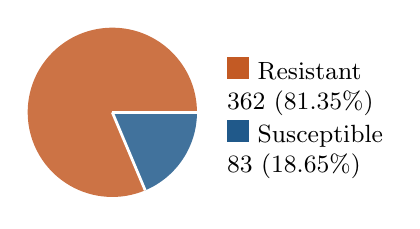
\begin{tikzpicture}[scale=0.86]
\fill[resorange!85] (0,0)--(0:1.25) arc (0:292.854:1.25)--cycle;
\fill[resblue!85] (0,0)--(292.854:1.25) arc (292.854:360:1.25)--cycle;
\draw[white,line width=1pt] (0,0)--(0:1.25);
\draw[white,line width=1pt] (0,0)--(292.854:1.25);
\node[font=\small,align=left,anchor=west] at (1.55,0.38) {\textcolor{resorange}{\rule{8pt}{8pt}} Resistant\\362 (81.35\%)};
\node[font=\small,align=left,anchor=west] at (1.55,-0.55) {\textcolor{resblue}{\rule{8pt}{8pt}} Susceptible\\83 (18.65\%)};
\end{tikzpicture}
\caption{Development-cohort composition ($n=445$). These proportions describe the retained study cohort, not population prevalence.}
\label{fig:pie}
\end{figure}

\subsection{Baselines and Implementation}
The initial comparison uses majority prediction, class-weighted logistic regression ($C=1$, liblinear solver), and 300-tree random-forest and Extra Trees models with minimum leaf size two. The saved V1 tuning search evaluates 28 configurations: four logistic-regression regularization values and 12 configurations for each tree-ensemble family. Its selected random forest is retained as the V2 control.

V2 includes that control, random forests and Extra Trees with minimum leaf sizes one, two, or four, logistic regression with $C\in\{0.1,1\}$, and histogram gradient boosting with seven or 15 maximum leaves. The latter uses 200 iterations, learning rate 0.05, minimum leaf size ten, and L2 regularization of one. Training uses scikit-learn~\cite{sklearn}; the saved V2 metadata records version 1.9.0 and NumPy 2.4.6. Randomized estimators use seed 42. This paper audits the existing run and predictions rather than reporting a new training run.

\subsection{Metrics and Evaluation Status}
Let $TP$ denote correctly predicted resistant isolates and $TN$ correctly predicted susceptible isolates. Then
\begin{equation}
\mathrm{Accuracy}=\frac{TP+TN}{TP+TN+FP+FN},
\end{equation}
\begin{equation}
\mathrm{BA}=\frac{1}{2}\left(\frac{TP}{TP+FN}+\frac{TN}{TN+FP}\right).
\end{equation}
Balanced accuracy (BA) gives equal weight to resistant and susceptible recall. We also report the area under the receiver operating characteristic curve (AUROC). Development summary values are unweighted means across the three folds, not metrics recomputed after pooling all isolates. The distinction is retained in every comparison.

The historical 114-isolate test partition was evaluated for V1, but its results subsequently informed development. It is therefore unsuitable as fresh independent validation of V2. V2 neither trains on nor re-evaluates this partition in the saved run. No confidence interval for external performance is inferred from only three development folds.

\section{Results and Discussion}
\subsection{Development Performance}
Table~\ref{tab:models} and Fig.~\ref{fig:bar} compare the saved development results. The selected V2 model reaches mean accuracy of 90.37\% and BA of 83.66\%. These values answer different questions: accuracy weights isolates equally, while BA weights the two classes equally. Majority prediction already reaches 81.54\% mean accuracy but has zero susceptible recall. Accuracy alone would conceal that failure.

\begin{table}[t]
\caption{Mean Development-Fold Performance (Percent)}
\label{tab:models}
\centering\footnotesize
\setlength{\tabcolsep}{3pt}
\begin{tabular}{lrrrrr}\toprule
Model & Acc. & BA & S recall & R recall & AUROC\\\midrule
Majority &81.54&50.00&0.00&100.00&50.00\\
Logistic regression &82.56&77.23&69.03&85.44&86.31\\
Random forest (initial)&84.37&78.56&69.43&87.68&85.47\\
Extra Trees (initial)&85.06&78.47&68.15&88.80&85.69\\
V1 control &88.10&83.09&75.51&90.68&86.95\\
V2 selected &\textbf{90.37}&\textbf{83.66}&73.35&93.98&87.10\\\bottomrule
\end{tabular}
\vspace{3pt}
\parbox{\columnwidth}{\footnotesize Acc.: accuracy; S: susceptible; R: resistant. V1 and V2 are selected configurations evaluated on reused development folds. Values are descriptive, not independent estimates of improvement.}
\end{table}

\begin{figure}[t]
\centering
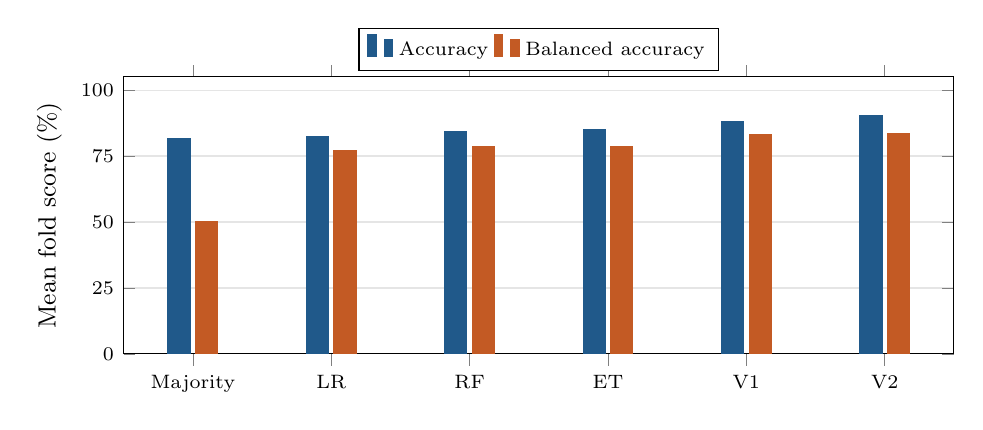
\begin{tikzpicture}
\begin{axis}[ybar,bar width=8pt,width=\columnwidth,height=5.1cm,ymin=0,ymax=105,ylabel={Mean fold score (\%)},symbolic x coords={Majority,LR,RF,ET,V1,V2},xtick=data,ytick={0,25,50,75,100},tick label style={font=\scriptsize},label style={font=\small},legend style={font=\scriptsize,at={(0.5,1.02)},anchor=south,legend columns=2},ymajorgrids,grid style={gray!20}]
\addplot[fill=resblue,draw=resblue] coordinates {(Majority,81.54)(LR,82.56)(RF,84.37)(ET,85.06)(V1,88.10)(V2,90.37)};
\addplot[fill=resorange,draw=resorange] coordinates {(Majority,50)(LR,77.23)(RF,78.56)(ET,78.47)(V1,83.09)(V2,83.66)};
\legend{Accuracy,Balanced accuracy}
\end{axis}
\end{tikzpicture}
\caption{Development performance. LR: logistic regression; RF: initial random forest; ET: initial Extra Trees. V1 and V2 include development-set selection.}
\label{fig:bar}
\end{figure}

Relative to the V1 control at threshold 0.50, V2 increases mean accuracy by 2.26 percentage points and BA by 0.57 points. Resistant recall rises from 90.68\% to 93.98\%, while susceptible recall falls from 75.51\% to 73.35\%. Both tree configuration and threshold change, so this comparison cannot attribute the difference to threshold adjustment alone. Nor does the small BA difference demonstrate a statistically established improvement.

\subsection{Between-Fold Variation}
Table~\ref{tab:folds} shows why a single mean score is insufficient. Fold 3 has BA of 67.15\% despite accuracy of 85.62\%. Only 10 of its 26 susceptible isolates are correctly classified, whereas 115 of 120 resistant isolates are correctly classified. Its class imbalance makes the accuracy look considerably stronger than its susceptible-class discrimination. Fold 1, by contrast, classifies 153 of 157 isolates correctly.

\begin{table}[t]
\caption{Selected V2 Model: Out-of-Fold Results}
\label{tab:folds}
\centering\footnotesize
\begin{tabular}{crrrrr}\toprule
Fold & $n$ & Acc. (\%) & BA (\%) & S recall (\%) & R recall (\%)\\\midrule
1&157&97.45&97.42&97.37&97.48\\
2&142&88.03&86.41&84.21&88.62\\
3&146&85.62&67.15&38.46&95.83\\\bottomrule
\end{tabular}
\end{table}

Fig.~\ref{fig:scatter} displays the saved resistant-class probabilities and the selected threshold. Horizontal displacement separates overlapping observations and has no biological meaning. The susceptible points above the threshold in fold 3 expose the failure that the mean accuracy obscures. These probabilities are not calibrated estimates of patient risk. The plot identifies disagreement with labels, not its biological cause; resolving that cause requires reviewing sequence evidence, phenotype provenance, and sampling composition.

\begin{figure}[t]
\centering
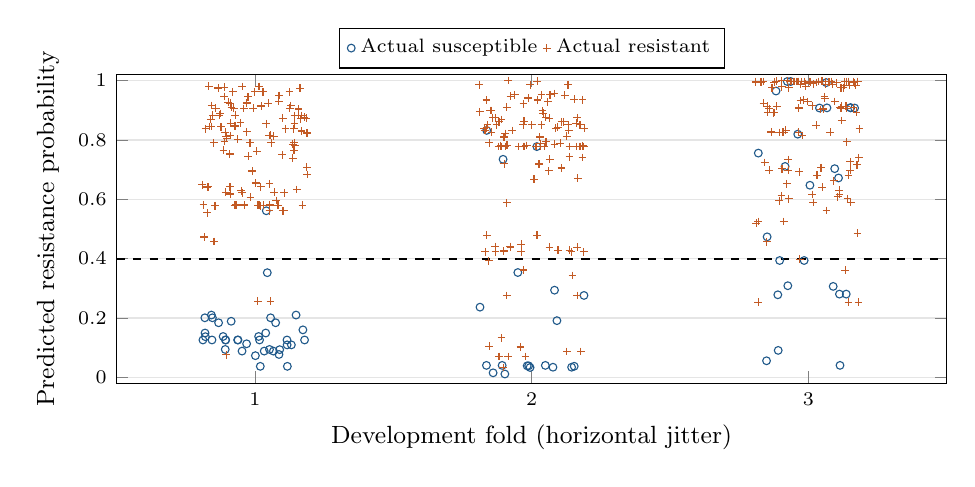
\begin{tikzpicture}
\begin{axis}[width=\columnwidth,height=5.5cm,xmin=0.5,xmax=3.5,ymin=-0.02,ymax=1.02,xtick={1,2,3},xlabel={Development fold (horizontal jitter)},ylabel={Predicted resistance probability},tick label style={font=\scriptsize},label style={font=\small},legend style={font=\scriptsize,at={(0.5,1.02)},anchor=south,legend columns=2},ymajorgrids,grid style={gray!20}]
\addplot[only marks,mark=o,mark size=1.4pt,color=resblue] coordinates {(1.05298,0.0939416) (0.81950,0.2005627) (0.91451,0.1888849) (0.89482,0.1257929) (1.08986,0.0931712) (1.06715,0.0883168) (1.14903,0.2097872) (0.84304,0.2097872) (0.97033,0.1129403) (0.82132,0.1368623) (0.89308,0.0939416) (1.00204,0.0729096) (0.82008,0.1492535) (0.88556,0.1375697) (1.05696,0.2005627) (1.01708,0.1257929) (0.89377,0.1257929) (1.03392,0.0883168) (1.11758,0.0369418) (0.81247,0.1257929) (1.11621,0.1257929) (1.07529,0.1838029) (0.93930,0.1257929) (0.86908,0.1838029) (1.17374,0.1598853) (0.93791,0.1257929) (0.84524,0.1257929) (0.84675,0.2005627) (1.13205,0.1092436) (1.03942,0.1492535) (1.11671,0.1092436) (1.08730,0.0769158) (1.01377,0.1375697) (1.17978,0.1257929) (0.95384,0.0883168) (1.01978,0.0369418) (1.04504,0.3525759) (1.04141,0.5613093) (1.89368,0.0401171) (1.83698,0.0401171) (2.04982,0.0401171) (1.89700,0.7348213) (2.15406,0.0372196) (1.98961,0.0386424) (2.01912,0.7776310) (1.99454,0.0330459) (2.08300,0.2936474) (1.90356,0.0110824) (1.98415,0.0386424) (2.18941,0.2759413) (1.83784,0.8322399) (2.14473,0.0339534) (1.95042,0.3531270) (2.07735,0.0339534) (1.86103,0.0150333) (2.09167,0.1909454) (1.81367,0.2363930) (3.11253,0.2804260) (3.13707,0.2804260) (2.88983,0.2780940) (2.84906,0.0556651) (3.08989,0.3064205) (2.93623,0.9970939) (3.10920,0.6718828) (2.98492,0.3936695) (2.92597,0.3086682) (2.89649,0.3936695) (2.88339,0.9649388) (2.91607,0.7107320) (2.96188,0.8194900) (2.85119,0.4734236) (3.04036,0.9076986) (3.06484,0.9933169) (2.92412,0.9970939) (3.16734,0.9076986) (3.06738,0.9081957) (3.15307,0.9081957) (2.89121,0.0906636) (3.15245,0.9092027) (3.00587,0.6473068) (3.09543,0.7032501) (2.81928,0.7556907) (3.11454,0.0402082)};
\addplot[only marks,mark=+,mark size=1.4pt,color=resorange] coordinates {(1.12517,0.9619797) (1.13745,0.7386471) (1.02939,0.9619797) (1.07774,0.5958795) (0.82741,0.6414110) (0.89660,0.0756914) (0.91997,0.9619797) (0.84032,0.8689170) (0.89846,0.8046359) (0.84838,0.8837496) (0.91563,0.9094943) (1.05156,0.8149306) (0.94864,0.8579206) (0.95067,0.6284223) (0.88961,0.9468159) (0.91145,0.8149306) (1.16593,0.8714677) (1.05625,0.8164559) (1.04147,0.8549410) (0.87503,0.8889323) (1.08707,0.9294762) (0.87209,0.8837496) (0.95419,0.6219590) (1.18602,0.8735736) (1.05320,0.5613093) (1.02164,0.6417212) (1.07015,0.6243610) (1.13028,0.9162193) (1.10488,0.5613093) (0.89704,0.8128155) (0.82220,0.8377258) (0.92987,0.5796745) (0.91174,0.8567716) (0.89017,0.9778111) (1.16831,0.8300770) (1.14302,0.8819946) (0.92958,0.8837496) (1.05907,0.7906928) (0.96034,0.9061851) (1.15753,0.9042048) (0.98436,0.6068075) (0.91065,0.9236034) (0.90372,0.9274985) (1.02332,0.9144272) (0.90984,0.6417212) (1.03214,0.5796745) (1.15117,0.6333015) (0.96177,0.5806825) (0.89334,0.8259351) (1.18906,0.6837738) (1.00362,0.6549757) (0.84455,0.9162193) (0.82790,0.5542096) (0.85167,0.7906928) (1.04843,0.9237844) (1.11099,0.8377258) (0.97042,0.9247157) (0.83414,0.9813618) (0.95502,0.9804546) (1.18853,0.8236216) (1.01106,0.2559493) (1.17901,0.8767863) (1.13710,0.7861620) (0.81436,0.5818829) (1.08387,0.5796745) (1.06905,0.8128155) (1.01405,0.5796745) (0.91139,0.6417212) (1.05357,0.5806825) (0.85239,0.4575692) (0.97521,0.9451059) (0.98242,0.7906928) (1.17245,0.5796745) (1.14282,0.7906928) (0.91009,0.7527827) (1.00022,0.9619797) (0.87789,0.8438604) (1.15680,0.8824765) (1.14080,0.8377258) (0.92341,0.9073749) (1.05280,0.6522000) (0.86808,0.9749900) (1.09975,0.5613093) (1.01496,0.5796745) (1.10588,0.6219590) (1.01153,0.5796745) (0.81022,0.6493364) (0.93318,0.5806825) (0.81740,0.4727315) (1.16306,0.9742079) (1.14391,0.7809245) (1.12603,0.9073749) (0.92686,0.5796745) (0.83201,0.6417212) (1.14364,0.8549410) (1.16984,0.8826332) (0.84255,0.8449445) (0.99468,0.9073749) (0.83630,0.8449445) (1.09903,0.7504770) (1.10102,0.8736385) (0.85879,0.9073749) (0.99061,0.6952920) (1.01893,0.5783929) (0.91072,0.6177567) (1.14152,0.7658367) (0.97079,0.8273917) (0.89048,0.7950689) (1.01493,0.9804546) (1.08737,0.9494761) (0.88644,0.7651800) (0.92845,0.8470103) (1.18816,0.7079523) (1.05695,0.2566921) (0.97648,0.7447099) (1.00668,0.7619416) (0.85598,0.5783929) (0.89538,0.6239541) (0.93847,0.8029949) (2.03356,0.7776310) (1.89744,0.0330459) (2.13666,0.7776310) (1.83693,0.9347234) (1.90044,0.8098330) (2.06421,0.8736531) (1.89141,0.8686373) (1.86028,0.8750207) (2.16550,0.8750207) (2.02700,0.7188545) (2.10816,0.8617102) (2.11685,0.8617102) (1.88236,0.8617102) (1.84683,0.7900356) (1.97380,0.7776310) (1.97096,0.3618257) (1.98747,0.9415647) (2.08705,0.8396603) (2.06588,0.7348213) (2.18398,0.7408878) (1.84740,0.1044944) (1.96300,0.4490357) (1.93893,0.9521059) (2.13744,0.4287506) (1.90449,0.8215725) (1.88228,0.0697078) (1.98047,0.7813411) (1.97032,0.7776310) (1.91585,0.0697078) (1.90493,0.7776310) (2.16084,0.8567636) (1.97839,0.0697078) (2.13731,0.7434626) (1.82922,0.8396603) (2.18973,0.8396603) (2.12769,0.0871930) (2.17822,0.0871930) (2.16202,0.7776310) (2.13250,0.8506395) (1.87320,0.8506395) (1.89122,0.7776310) (1.96240,0.4234994) (1.83228,0.4234994) (1.95401,0.7776310) (2.18442,0.9352095) (1.91078,0.5887480) (2.10795,0.7055402) (1.98290,0.7813411) (1.97074,0.7776310) (2.17378,0.7776310) (2.18826,0.7776310) (2.02119,0.9347234) (1.86882,0.4406943) (1.92275,0.4406943) (2.17811,0.7776310) (2.03009,0.8098330) (2.01603,0.7776310) (2.09423,0.8434740) (1.83172,0.8322399) (2.03199,0.7879507) (2.00108,0.8506395) (2.13403,0.8322399) (1.86982,0.8750207) (2.17510,0.8506395) (1.84044,0.8506395) (1.88061,0.7776310) (2.03611,0.9521059) (2.06658,0.9521059) (1.89938,0.4258842) (1.85556,0.8260679) (2.14831,0.3433484) (2.03592,0.8506395) (2.04536,0.7776310) (1.96931,0.8506395) (2.03180,0.7776310) (2.00866,0.6681984) (2.16519,0.4383167) (1.88762,0.7776310) (2.08215,0.9567183) (1.90070,0.7201045) (1.96040,0.1019947) (2.06524,0.4383167) (1.92400,0.4383167) (1.93015,0.8322399) (2.09571,0.4287506) (1.83757,0.8409233) (2.18852,0.4234994) (1.89100,0.1326580) (1.91078,0.2759413) (2.16464,0.2759413) (2.14412,0.4234994) (1.86994,0.4234994) (2.12682,0.8123230) (2.04244,0.8904411) (2.18515,0.7800727) (2.05851,0.9281814) (1.81297,0.8954239) (2.12050,0.9513136) (1.92376,0.9474791) (2.06209,0.6956128) (2.16679,0.6711354) (1.85386,0.8996383) (1.85067,0.8996383) (2.02022,0.9976528) (1.91349,0.7826021) (2.03984,0.8987563) (2.08269,0.7851817) (1.88737,0.7810929) (2.05101,0.8765751) (1.91031,0.9105640) (1.99564,0.9854311) (2.15403,0.9371361) (2.13152,0.9860056) (1.84507,0.3922078) (1.97096,0.9223770) (1.91514,1.0000000) (1.81135,0.9860056) (2.10303,0.7892136) (2.05210,0.7938065) (1.90954,0.7825624) (2.01964,0.4787187) (1.97252,0.8628647) (1.83859,0.4787187) (3.14558,0.6812836) (3.15349,0.5887692) (3.01732,0.5887692) (3.12715,0.9757956) (3.03135,0.6812836) (2.86628,0.8268930) (2.85843,0.6982483) (2.92714,0.6982483) (3.15161,0.6982483) (3.15159,0.7267329) (2.90482,0.7032501) (3.10644,0.6082306) (3.14597,0.9970939) (2.96442,0.8264347) (3.04585,0.7062441) (2.86873,0.9755839) (3.16335,0.9970939) (3.13855,0.7942077) (3.18096,0.2525591) (3.11809,0.9755839) (3.14494,0.2525591) (2.81942,0.2525591) (3.16371,0.9088424) (3.11485,0.9088424) (3.13834,0.9070582) (3.11808,0.9064332) (2.91139,0.5253490) (2.85108,0.9138434) (3.14142,0.6021952) (3.13627,0.9138434) (2.89452,0.5951103) (3.12030,0.9138434) (3.11223,0.6306439) (2.81899,0.5253490) (2.93474,0.9970939) (3.13845,0.9970939) (3.17742,0.4851943) (3.05376,0.9044525) (3.18284,0.7399445) (3.01376,0.9147233) (3.16691,0.9928542) (2.85383,0.8928844) (3.17875,0.9970939) (2.87786,0.8928844) (3.17576,0.7167184) (2.91088,0.8264347) (2.97513,0.9970939) (3.08685,0.9882050) (2.92920,0.9757956) (3.00434,0.9970939) (2.95637,0.9970939) (3.02910,0.8499028) (2.90679,0.8261966) (3.07934,0.8264347) (2.81064,0.9953333) (3.16172,0.9953333) (3.01461,0.6163751) (3.08338,0.9970939) (3.09194,0.6628148) (2.94840,0.9970939) (2.83659,0.9970939) (3.06241,0.9970939) (2.93548,0.9970939) (2.92929,0.6021952) (3.13225,0.9970939) (3.08351,0.9970939) (2.92753,0.7342417) (2.96519,0.9076986) (2.96291,0.9970939) (2.92235,0.6520613) (2.85837,0.9056292) (2.96977,0.3979136) (3.04390,0.9030197) (2.92436,1.0000000) (3.01822,0.9898546) (2.81015,0.9970939) (2.91903,0.8324123) (2.97336,0.9868549) (3.03039,0.9933169) (3.05879,0.9455747) (2.98670,0.9970939) (2.97802,0.8150996) (2.98981,0.9899836) (3.11249,0.6163751) (2.87448,0.8916301) (2.84222,0.7242555) (3.05052,0.6408030) (2.93737,0.9970939) (3.12100,0.8658945) (3.06566,0.5623755) (2.89536,0.8252334) (2.88567,0.9138900) (2.90304,0.6117174) (2.99055,0.9803829) (3.13290,0.3604541) (2.83767,0.9237333) (2.96749,0.6924354) (3.04931,0.9977433) (2.88389,0.9975052) (3.07461,0.9956228) (2.99786,0.9299252) (2.90271,1.0000000) (3.05930,0.9401011) (2.81211,0.5189922) (3.09537,0.9298400) (3.10262,0.9926851) (2.85050,0.4564851) (2.97156,0.9329750) (2.87684,0.9940991) (3.17403,0.8934693) (3.00682,0.9955000) (2.82908,0.9949841) (2.90470,0.9795857) (3.13237,0.9843702) (2.98346,0.9350500) (3.06368,0.9878796) (3.18540,0.8374978) (3.03627,0.9970939) (3.17102,0.9834281) (3.14874,0.9834281)};
\addplot[black,dashed,thick,forget plot] coordinates {(0.5,0.4)(3.5,0.4)};
\legend{Actual susceptible,Actual resistant}
\end{axis}
\end{tikzpicture}
\caption{Out-of-fold predictions for all 445 development isolates. The dashed line is the selected threshold of 0.40. Horizontal jitter is for visibility only.}
\label{fig:scatter}
\end{figure}

An additional saved feature experiment included partial and contig-end calls. Mean BA changed from 78.47\% to 78.61\% for the initial Extra Trees model, but decreased from 77.23\% to 76.31\% for logistic regression and from 78.56\% to 77.63\% for the initial random forest. Those development comparisons do not establish a consistent benefit from adding incomplete calls.

\subsection{Historical Benchmark and Sequence Feasibility}
The historical V1 test matrix contains 39 correctly classified susceptible isolates, two susceptible isolates classified as resistant, 12 resistant isolates classified as susceptible, and 61 correctly classified resistant isolates. Thus, 100 of 114 predictions were correct: accuracy was 87.72\%, BA 89.34\%, and AUROC 97.53\%. These are V1 historical results, not the V2 development scores and not current external validation. High ranking performance also did not eliminate threshold-dependent false-susceptible predictions.

The sequence pilot completed processing for ten development isolates: five public assemblies and five read-derived assemblies. All ten received feature reports. Subsequent read-mapping checks reported primary mapping of 97.70--99.22\%, mean aligned depth of 23.28--72.66, and assembly breadth at depth at least ten of 97.73--99.9988\%. These are technical checks against each sample's own assembly; they do not prove sample purity or complete genome recovery.

One pilot read set had uniform Q30 values in the sampled first 1,000 reads of each mate. The source-quality flag was retained instead of interpreting the reported Q30 fraction as perfect sequencing. The saved assembly-stage checkpoint records 310 existing-assembly reports plus five pilot read reports, or 315 genomes with features out of 445 development isolates. It also records seven assembly warnings, 130 remaining read samples, and a pending contamination screen. This checkpoint is a processing result; no prediction accuracy was measured for the regenerated feature set.

\subsection{Limitations and Surveillance Interpretation}
The cohort is small, resistance-enriched, and assembled from heterogeneous public projects. Requiring available genotype calls excludes records without such results. Removing 290 overlapping candidates changes the evaluated population and limits comparison with unrestricted random splits. BioProject and known-cluster separation cannot rule out unrecorded shared ancestry. Deposited CLSI labels also do not establish a uniform testing method or breakpoint edition across laboratories.

The feature representation captures reported genes and point mutations, but does not explicitly quantify gene expression, copy number, or all regulatory and structural variation. Database versions may change feature calls. Repeated development-set comparisons create selection optimism even when preprocessing is fitted within each fold. Finally, the present experiment evaluates isolate-level classification; it does not measure outbreak detection, alert lead time, geographic forecasting, treatment benefit, or prospective clinical turnaround time. The framework can organize evidence for surveillance review, but those operational outcomes require separate validation.

\section{Conclusion}
ResistMap AI provides an auditable workflow for linking genomic resistance calls to ceftazidime susceptibility in \kp{}. On three project-separated development folds, the selected random forest achieved 90.37\% mean accuracy and 83.66\% balanced accuracy. The 67.15--97.42\% fold-level BA range demonstrates that the average does not describe uniform performance across held-out projects. Sequence processing was feasible in a ten-genome pilot, but the regenerated features have not yet been evaluated as a trained predictor. The next study should freeze the complete feature pipeline, model, and threshold before testing on a newly acquired, independent cohort with documented phenotype methods and sequence quality.

\begin{thebibliography}{00}
\bibitem{burden} Antimicrobial Resistance Collaborators, ``Global burden of bacterial antimicrobial resistance in 2019: a systematic analysis,'' \textit{The Lancet}, vol. 399, pp. 629--655, 2022, doi: \href{https://doi.org/10.1016/S0140-6736(21)02724-0}{10.1016/S0140-6736(21)02724-0}.
\bibitem{kleborate} M. M. C. Lam \textit{et al.}, ``A genomic surveillance framework and genotyping tool for Klebsiella pneumoniae and its related species complex,'' \textit{Nature Communications}, vol. 12, art. 4188, 2021, doi: \href{https://doi.org/10.1038/s41467-021-24448-3}{10.1038/s41467-021-24448-3}.
\bibitem{nguyen} M. Nguyen \textit{et al.}, ``Developing an in silico minimum inhibitory concentration panel test for Klebsiella pneumoniae,'' \textit{Scientific Reports}, vol. 8, art. 421, 2018, doi: \href{https://doi.org/10.1038/s41598-017-18972-w}{10.1038/s41598-017-18972-w}.
\bibitem{leakage} S. Kapoor and A. Narayanan, ``Leakage and the reproducibility crisis in machine-learning-based science,'' \textit{Patterns}, vol. 4, no. 9, art. 100804, 2023, doi: \href{https://doi.org/10.1016/j.patter.2023.100804}{10.1016/j.patter.2023.100804}.
\bibitem{amrfinder} M. Feldgarden \textit{et al.}, ``AMRFinderPlus and the Reference Gene Catalog facilitate examination of the genomic links among antimicrobial resistance, stress response, and virulence,'' \textit{Scientific Reports}, vol. 11, art. 12728, 2021, doi: \href{https://doi.org/10.1038/s41598-021-91456-0}{10.1038/s41598-021-91456-0}.
\bibitem{resfinder} V. Bortolaia \textit{et al.}, ``ResFinder 4.0 for predictions of phenotypes from genotypes,'' \textit{Journal of Antimicrobial Chemotherapy}, vol. 75, no. 12, pp. 3491--3500, 2020, doi: \href{https://doi.org/10.1093/jac/dkaa345}{10.1093/jac/dkaa345}.
\bibitem{card} B. P. Alcock \textit{et al.}, ``CARD 2023: expanded curation, support for machine learning, and resistome prediction at the Comprehensive Antibiotic Resistance Database,'' \textit{Nucleic Acids Research}, vol. 51, no. D1, pp. D690--D699, 2023, doi: \href{https://doi.org/10.1093/nar/gkac920}{10.1093/nar/gkac920}.
\bibitem{curation} M. Feldgarden \textit{et al.}, ``Curation of the AMRFinderPlus databases: applications, functionality and impact,'' \textit{Microbial Genomics}, vol. 8, no. 6, art. 000832, 2022, doi: \href{https://doi.org/10.1099/mgen.0.000832}{10.1099/mgen.0.000832}.
\bibitem{macesic} N. Macesic \textit{et al.}, ``Predicting phenotypic polymyxin resistance in Klebsiella pneumoniae through machine learning analysis of genomic data,'' \textit{mSystems}, vol. 5, no. 3, art. e00656-19, 2020, doi: \href{https://doi.org/10.1128/mSystems.00656-19}{10.1128/mSystems.00656-19}.
\bibitem{mic} G. Batisti Biffignandi \textit{et al.}, ``Optimising machine learning prediction of minimum inhibitory concentrations in Klebsiella pneumoniae,'' \textit{Microbial Genomics}, vol. 10, no. 3, art. 001222, 2024, doi: \href{https://doi.org/10.1099/mgen.0.001222}{10.1099/mgen.0.001222}.
\bibitem{jia} X. Jia \textit{et al.}, ``Machine learning-based prediction of multi-level antimicrobial resistance in Klebsiella pneumoniae using whole-genome sequencing data,'' \textit{International Journal of Antimicrobial Agents}, vol. 67, no. 7, art. 107807, 2026, doi: \href{https://doi.org/10.1016/j.ijantimicag.2026.107807}{10.1016/j.ijantimicag.2026.107807}.
\bibitem{rf} L. Breiman, ``Random forests,'' \textit{Machine Learning}, vol. 45, pp. 5--32, 2001, doi: \href{https://doi.org/10.1023/A:1010933404324}{10.1023/A:1010933404324}.
\bibitem{extra} P. Geurts, D. Ernst, and L. Wehenkel, ``Extremely randomized trees,'' \textit{Machine Learning}, vol. 63, pp. 3--42, 2006, doi: \href{https://doi.org/10.1007/s10994-006-6226-1}{10.1007/s10994-006-6226-1}.
\bibitem{fastp} S. Chen, Y. Zhou, Y. Chen, and J. Gu, ``fastp: an ultra-fast all-in-one FASTQ preprocessor,'' \textit{Bioinformatics}, vol. 34, no. 17, pp. i884--i890, 2018, doi: \href{https://doi.org/10.1093/bioinformatics/bty560}{10.1093/bioinformatics/bty560}.
\bibitem{skesa} A. Souvorov, R. Agarwala, and D. J. Lipman, ``SKESA: strategic k-mer extension for scrupulous assemblies,'' \textit{Genome Biology}, vol. 19, art. 153, 2018, doi: \href{https://doi.org/10.1186/s13059-018-1540-z}{10.1186/s13059-018-1540-z}.
\bibitem{minimap} H. Li, ``Minimap2: pairwise alignment for nucleotide sequences,'' \textit{Bioinformatics}, vol. 34, no. 18, pp. 3094--3100, 2018, doi: \href{https://doi.org/10.1093/bioinformatics/bty191}{10.1093/bioinformatics/bty191}.
\bibitem{samtools} P. Danecek \textit{et al.}, ``Twelve years of SAMtools and BCFtools,'' \textit{GigaScience}, vol. 10, no. 2, art. giab008, 2021, doi: \href{https://doi.org/10.1093/gigascience/giab008}{10.1093/gigascience/giab008}.
\bibitem{sklearn} F. Pedregosa \textit{et al.}, ``Scikit-learn: Machine learning in Python,'' \textit{Journal of Machine Learning Research}, vol. 12, pp. 2825--2830, 2011. [Online]. Available: \url{https://jmlr.org/papers/v12/pedregosa11a.html}
\end{thebibliography}
\end{document}
